\documentclass{standalone}

\usepackage{pgf}
\usepackage{tikz}
\usetikzlibrary{arrows,automata,positioning,shapes.multipart}

\tikzset{every loop/.style={min distance=18mm}}
\tikzset{node distance=8cm,
	every state/.style={
		semithick,
		fill=gray!10,
		minimum size=2.5cm
	},
	initial text={},
	double distance=2pt,
	every edge/.style={
		draw,
		->,>=stealth',
		auto,
		semithick
	}
}

\begin{document}
	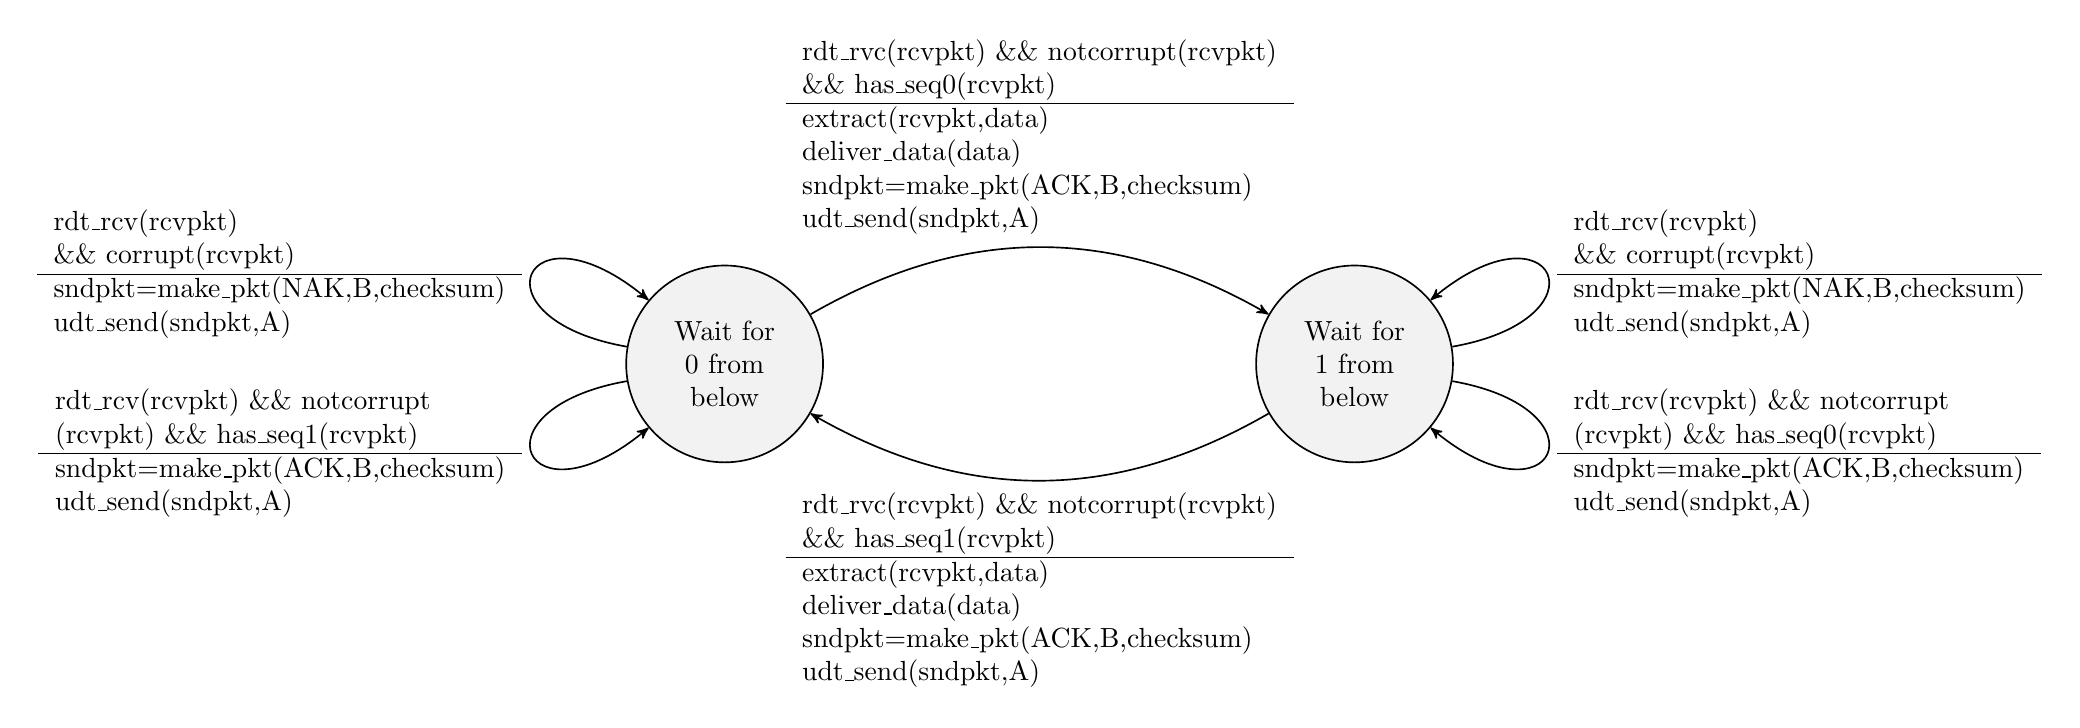
\begin{tikzpicture}[every text node part/.style={align=center}]
		\node[state] (call0) {Wait for\\0 from\\below};
		\node[state, right of=call0] (call1) {Wait for\\1 from\\below};
		
		\draw (call0) edge[out=170,in=140,loop] node[left]{
			\begin{tabular}{l}
				rdt\_rcv(rcvpkt)\\
				\&\& corrupt(rcvpkt)\\
				\hline
				sndpkt=make\_pkt(NAK,B,checksum)\\
				udt\_send(sndpkt,A)
			\end{tabular}} (call0);
		\draw (call0) edge[out=190,in=220,loop] node[left]{
			\begin{tabular}{l}
				rdt\_rcv(rcvpkt) \&\& notcorrupt\\
				(rcvpkt) \&\& has\_seq1(rcvpkt)\\
				\hline
				sndpkt=make\_pkt(ACK,B,checksum)\\
				udt\_send(sndpkt,A)
			\end{tabular}} (call0);

		\draw (call0) edge[bend left] node{
			\begin{tabular}{l}
				rdt\_rvc(rcvpkt) \&\& notcorrupt(rcvpkt)\\
				\&\& has\_seq0(rcvpkt)\\
				\hline
				extract(rcvpkt,data)\\
				deliver\_data(data)\\
				sndpkt=make\_pkt(ACK,B,checksum)\\
				udt\_send(sndpkt,A)
			\end{tabular}} (call1);

		\draw (call1) edge[out=10,in=40,loop] node[right]{
			\begin{tabular}{l}
				rdt\_rcv(rcvpkt)\\
				\&\& corrupt(rcvpkt)\\
				\hline
				sndpkt=make\_pkt(NAK,B,checksum)\\
				udt\_send(sndpkt,A)
			\end{tabular}} (call1);
		\draw (call1) edge[out=350,in=320,loop] node[right]{
			\begin{tabular}{l}
				rdt\_rcv(rcvpkt) \&\& notcorrupt\\
				(rcvpkt) \&\& has\_seq0(rcvpkt)\\
				\hline
				sndpkt=make\_pkt(ACK,B,checksum)\\
				udt\_send(sndpkt,A)
			\end{tabular}} (call1);

		\draw (call1) edge[bend left] node{
			\begin{tabular}{l}
				rdt\_rvc(rcvpkt) \&\& notcorrupt(rcvpkt)\\
				\&\& has\_seq1(rcvpkt)\\
				\hline
				extract(rcvpkt,data)\\
				deliver\_data(data)\\
				sndpkt=make\_pkt(ACK,B,checksum)\\
				udt\_send(sndpkt,A)
			\end{tabular}} (call0);

	\end{tikzpicture}
\end{document}
